\documentclass[a4paper]{article}

\usepackage[english]{babel}
\usepackage[utf8]{inputenc}
\usepackage{apacite}
\usepackage{graphicx}
\usepackage{tikz}
\usetikzlibrary{positioning}
\usepackage{xcolor}
\usepackage[colorinlistoftodos]{todonotes}
\usepackage{enumitem}
\setitemize{noitemsep,topsep=0pt,parsep=0pt,partopsep=0pt}

\makeatletter
\def\BState{\State\hskip-\ALG@thistlm}
\makeatother

\title{Gameplay Design \\ Assignment 2 \\ Analysis of \textit{7 Wonders} and \textit{Ricocheting Robots} }

\author{
  Bowald, Johan\\
  \texttt{bowaldj@student.chalmers.se}
  \and
  Odbjer, Sebastian\\
  \texttt{sebastian.odbjer@gmail.com}
}

\date{\today}

\tikzset{
    vertex/.style = {
        circle,
        fill  = black,
        outer sep = 2pt,
        inner sep = 1pt,
    }
}

\begin{document}
\maketitle
\newpage
\tableofcontents{}
\newpage

\section{Gameplay description 7 Wonders}
\label{sec:what7wond}
7 Wonders was released in 2010 and the goal is to build a civilisation in an ancient setting.
The game consist of several card types and a player unique game board showing the status of a player's civilisation.
The different cards represent different buildings which each contribute to the civilisation in some way.
There are resource spawning, such as iron, chemicals or wood. Military cards which are used to battle with one's neighbours, these battles give points to the victors and deduct points from the losers.
Science Cards, which generate points at the end of the game. There are three different science cards, each with a unique scientific tool.
The amount of points given by science cards is based on the amount of complete science tool sets that has been collected as well as the number of cards you have of each unique science tool type.
Another card type is what we have chosen to call utility cards, they have an immediate effect on the game state.
These cards are either played to collect money instantaneously or used to establish trading posts that give discounts while trading with one's neighbours.
The last card type is point cards.
They either consist of buildings that gives a fixed amount of points or dynamic point cards that are given points based on ones own and neighbouring civilisation statuses.
The game is divided into three ages, each age is divided into six turns.
Each turn every player picks a card which is either played, discarded or used as a resource to build a wonder.
Wonders have different impact on the game, they can either generate resources, points, science, currency or military power.
The effect of wonders are unique for each civilisation.
The rest of the cards are passed to the next player in a drafting fashion.
To play a card some resources must be paid, they can either be resources generated by ones own civilisation or they can be bought from neighbouring civilisations, provided they possess them.
After the three ages have passed points are counted for each player's success in each card type area, such as military, science and point cards.
The amount of currency currently in each player's possession is also counted and rewarded with points.
The player that has the most points at the end wins the game.

\subsection{Gameplay of 7 Wonders using the component framework}
In this section we are breaking down the gameplay elements of 7 wonders by using the component framwork \cite{bjork2003describing}.
\subsubsection{A typical gameinstance of 7 wonders}

\begin{itemize}[noitemsep,topsep=0pt,parsep=0pt,partopsep=0pt]
  \item Which cards that a specific game should use is decided by the number of players
  \item Players chooses civilisation by picking a player unique gameboard
  \item Cards are shuffled and each player receives seven cards from the first age
  \item Drafting session
  \item Cards are shuffle and each player receives seven cards from the second age
  \item Drafting session
  \item Cards are shuffle and each player receives seven cards from the third age
  \item Drafting session
  \item Outcome is determined by counting points based on card types and currency
  \item Clearing the game state
\end{itemize}

\subsubsection{A typical game session of 7 wonders}
\begin{itemize}[noitemsep,topsep=0pt,parsep=0pt,partopsep=0pt]
  \item Pick civilisation
  \item Draft of the first age
  \item Pick a card, chose to play, discard or build wonder. Pass the rest of the cards to opponent.
  \item Drafting session of the second age
  \item Pick a card, chose to play, discard or build wonder. Pass the rest of the cards to opponent.
  \item Drafting session of the third age
  \item Pick a card, chose to play, discard or build wonder. Pass the rest of the cards to opponent.
\end{itemize}

\subsubsection{A typical player session of 7 wonders}
In this game the player session is the same as the game session. All player sessions are played simultaneously due to the drafting mechanic.

\subsubsection{Goals and subgoals}
\begin{itemize}[noitemsep,topsep=0pt,parsep=0pt,partopsep=0pt]
  \item Get as high score as possible
  \item Complete scientific tool sets
  \item Gathere as many scientific cards of the same type as possible
  \item Have higher military power then the neighbours
  \item Complete the civilisations wonder
  \item Get a high score by stratigically timing the dynamic point cards
  \item Have enough resources to play the perfect cards
\end{itemize}
\section{Gameplay description Ricocheting Robots}
Ricochet robots is a game where players challenge each other to move a robot to a certain point.
The game consists of a board with a grid layout. Some of the grid tiles are unique goal tile.
The goal tiles have a color matching one of the robots(except the optional support robot) and a symbol.
The board also have walls placed between some tiles. A robot cannot move through these walls, instead they ricochet along the wall in the direction of the players choice.
Each turn a random goal token is revealed.
Then each player simentainusly tries to figure out the path with the fewest moves to move the robot with corresponding color as goal token to the goal tile indicated by the goal token. 

When one player have found a legit path, that player state the amount of movements required to carry out the task.
The other players have one minute to try to beat the first player number of movements. When the time ends, that player with the fewest movements gets the point and a new turn begins.
A player can bid a higher amount of movements in case the player with the original bid cannot show his solution.
When all goal tokens are collected by the players, the player with the most goal tokens wins the game.

\section{Analysis using game design patterns}
We have analysed using Game Design patterns framework \cite{Bjork2003}.
Some of the patterns are fetched from the wikipedia for Gameplay Design Patterns \url{gdp2.tii.se}.
Others are defined by us.
At the end of this section a comparison of both games is presented.
One weakness of the Game design patterns is that every pattern either needs to be redefined in every analysis so it can not be misinterpreted or universally defined(in a database or wiki).
One negative thing about universally defining patterns is that people could partially lose track of their own analysis of the gameplay.
Instead they might try to make certain predefined patterns fit, as if trying to fit a piece into a puzzle, while possibly missing other key patterns.

\newpage
\subsection{7 Wonders analysis}
\begin{figure}[htb]

\centering
  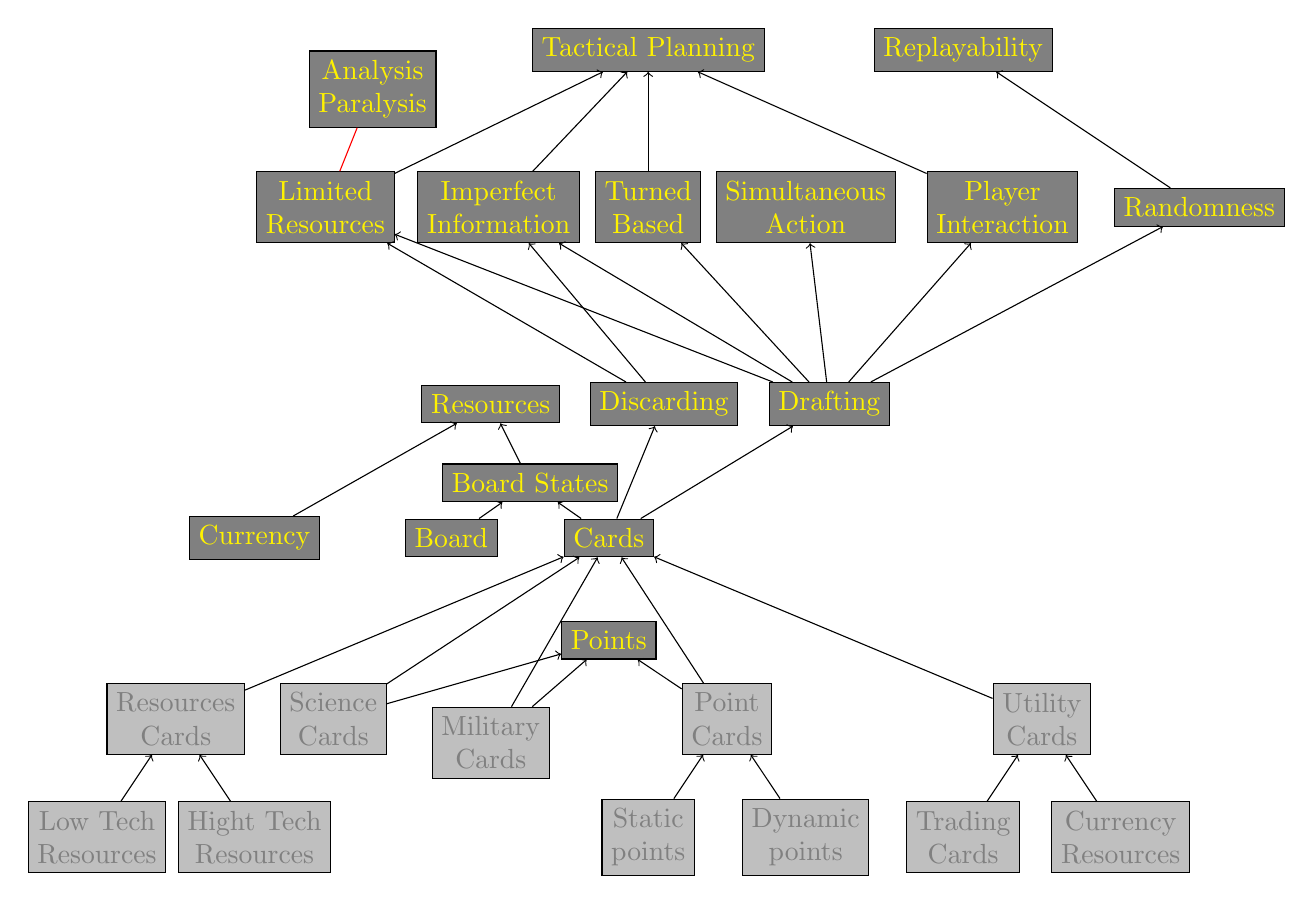
\begin{tikzpicture}

  \node[draw,fill=gray!50,text=gray, align=center] (LTRe) at (-6,0) {Low Tech\\ Resources};
  \node[draw,fill=gray!50,text=gray, align=center] (HTRe) at (-4,0){Hight Tech\\ Resources};

  \node[draw,fill=gray!50,text=gray, align=center] (CuRe) at (7,0) {Currency \\Resources};
  \node[draw,fill=gray!50,text=gray, align=center] (TrCa) at (5,0) {Trading \\Cards};  

  \node[draw,fill=gray!50,text=gray, align=center] (StPo) at (1,0) {Static\\points};
  \node[draw,fill=gray!50,text=gray, align=center] (DyPo) at (3,0) {Dynamic\\points};
  
  \node[draw,fill=gray!50,text=gray, align=center] (ReCa) at (-5,1.5) {Resources\\ Cards};
  \draw[->,draw=black] (LTRe) to (ReCa);
  \draw[->,draw=black] (HTRe) to (ReCa);
  \node[draw,fill=gray!50,text=gray, align=center] (ScCa) at (-3,1.5) {Science\\Cards};
  \node[draw,fill=gray!50,text=gray, align=center] (MiCa) at (-1,1.2) {Military\\Cards};
  \node[draw,fill=gray!50,text=gray, align=center] (PoCa) at (2,1.5) {Point\\Cards};
  \draw[->,draw=black] (DyPo) to (PoCa);
  \draw[->,draw=black] (StPo) to (PoCa);
  \node[draw,fill=gray!50,text=gray, align=center] (UtCa) at (6,1.5) {Utility\\Cards};
  \draw[->,draw=black] (TrCa) to (UtCa);
  \draw[->,draw=black] (CuRe) to (UtCa);

  \node[draw,fill=gray,text=yellow] (Po) at (0.5,2.5) {Points};

  \draw[->,draw=black] (ScCa) to (Po);
  \draw[->,draw=black] (MiCa) to (Po);
  \draw[->,draw=black] (PoCa) to (Po);

  \node[draw,fill=gray,text=yellow] (Ca) at (0.5,3.8) {Cards};

  \draw[->,draw=black] (ScCa) to (Ca);
  \draw[->,draw=black] (MiCa) to (Ca);
  \draw[->,draw=black] (PoCa) to (Ca);
  \draw[->,draw=black] (ReCa) to (Ca);
  \draw[->,draw=black] (UtCa) to (Ca);
  
  % \node[draw,fill=gray!50,text=gray, align=center ](PoTo) {Point\\Tokens};
  \node[draw,fill=gray,text=yellow] (Cu) at (-4,3.8){Currency};
  \node[draw,fill=gray,text=yellow] (Bo) at (-1.5,3.8){Board};


  % %to points, resources
  \node[draw,fill=gray,text=yellow] (BoSt) at (-0.5,4.5) {Board States};
  \draw[->,draw=black] (Bo) to (BoSt);
  \draw[->,draw=black] (Ca) to (BoSt);

  \node[draw,fill=gray,text=yellow] (Re) at (-1,5.5) {Resources};
  \node[draw,fill=gray,text=yellow] (Di) at (1.2,5.5) {Discarding};
  \node[draw,fill=gray,text=yellow] (Da) at (3.3,5.5) {Drafting};
  \draw[->,draw=black] (Cu) to (Re);
  \draw[->,draw=black] (BoSt) to (Re);
  \draw[->,draw=black] (Ca) to (Da);
  \draw[->,draw=black] (Ca) to (Di);

  % %Drafting, discarding
  \node[draw,fill=gray,text=yellow, align=center] (ImIn) at (-0.9,8) {Imperfect\\Information};
  \node[draw,fill=gray,text=yellow, align=center] (LiRe) at (-3.1,8) {Limited\\Resources};
  \node[draw,fill=gray,text=yellow, align=center] (TuBa) at (1,8) {Turned\\Based};
  \node[draw,fill=gray,text=yellow, align=center] (SiAc) at (3,8) {Simultaneous\\Action};
  \node[draw,fill=gray,text=yellow, align=center] (PlIn) at (5.5,8) {Player\\Interaction};
  \node[draw,fill=gray,text=yellow, align=center] (Ra) at (8,8) {Randomness};

  \draw[->,draw=black] (Di) to (ImIn);
  \draw[->,draw=black] (Di) to (LiRe);

  \draw[->,draw=black] (Da) to (ImIn);
  \draw[->,draw=black] (Da) to (LiRe);
  \draw[->,draw=black] (Da) to (TuBa);
  \draw[->,draw=black] (Da) to (SiAc);
  \draw[->,draw=black] (Da) to (PlIn);
  \draw[->,draw=black] (Da) to (Ra);

  % %Drafting trading cards
  
  \node[draw,fill=gray,text=yellow, align=center] (AnPa) at (-2.5,9.5){Analysis\\Paralysis};
  \draw[-,draw=red] (LiRe) to (AnPa);
  \node[draw,fill=gray,text=yellow] (TaPl) at (1,10){Tactical Planning};
  \node[draw,fill=gray,text=yellow] (Re) at (5,10){Replayability};
  \draw[->,draw=black] (ImIn) to (TaPl);
  \draw[->,draw=black] (LiRe) to (TaPl);
  \draw[->,draw=black] (TuBa) to (TaPl);
  \draw[->,draw=black] (PlIn) to (TaPl);
  \draw[->,draw=black] (Ra) to (Re);

  % \node[draw,fill=gray,text=yellow] (KiMa) {King Maker};

  \end{tikzpicture}
\caption{Analysis of 7 Wonders using Game Design Pattern.
Light gray boxes indicates gameplay mechanics unique to 7 Wonders.
Dark gray boxes are abstract mechanics found in other games.
Edges with arrows indicate that the pattern being pointed to is instantiated by the other pattern connected to the edge.
Red edges indicates that at pattern is in conflict with another pattern.}

\label{fig:A7W}
\end{figure}

\newpage
\subsection{Ricocheting Robots analysed using Game Design Patterns}
% Ricocheting Robots Game pattern analysis
\begin{figure}[htb]
\centering
  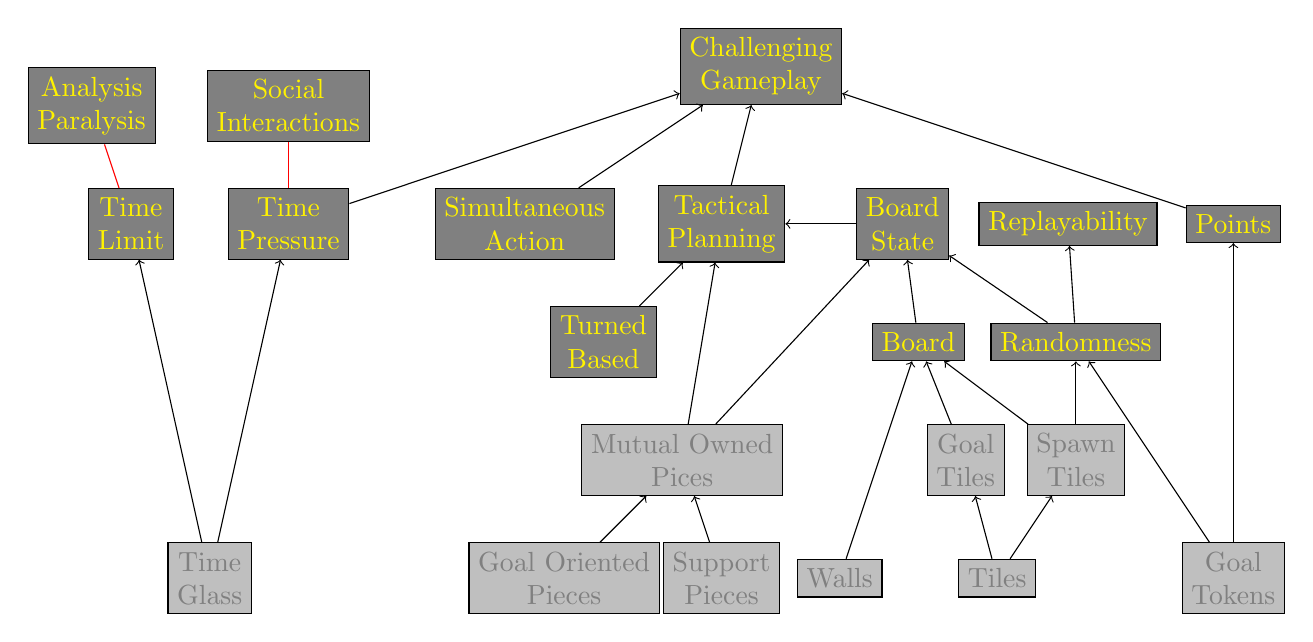
\begin{tikzpicture}

    \node[draw,fill=gray!50,text=gray, align=center] (TiGl) at (-6,0) {Time\\Glass};

    \node[draw,fill=gray!50,text=gray, align=center] (GOPi) at (-1.5,0) {Goal Oriented\\Pieces};
    \node[draw,fill=gray!50,text=gray, align=center] (SuPi) at (0.5,0) {Support\\Pieces};
    
    \node[draw,fill=gray!50,text=gray, align=center] (Wa) at (2,0) {Walls};
    \node[draw,fill=gray!50,text=gray, align=center] (Ti) at (4,0) {Tiles};

    \node[draw,fill=gray!50,text=gray, align=center] (GoTo) at (7,0) {Goal\\Tokens};  

    \node[draw,fill=gray!50,text=gray, align=center] (MOPi) at (0,1.5) {Mutual Owned\\Pices};
    \node[draw,fill=gray!50,text=gray, align=center] (GoTi) at (3.6,1.5) {Goal\\Tiles};
    \node[draw,fill=gray!50,text=gray, align=center] (SpTi) at (5,1.5) {Spawn\\Tiles};

    \node[draw,fill=gray,text=yellow, align=center] (Bo) at (3,3) {Board};
    \node[draw,fill=gray,text=yellow, align=center] (Ra) at (5,3) {Randomness};
    \node[draw,fill=gray,text=yellow, align=center] (TuBa) at (-1,3) {Turned\\Based};

    \node[draw,fill=gray,text=yellow, align=center] (TiLi) at (-7,4.5) {Time\\Limit};
    \node[draw,fill=gray,text=yellow, align=center] (TiPr) at (-5,4.5) {Time\\Pressure};
    \node[draw,fill=gray,text=yellow, align=center] (Re) at (4.9,4.5) {Replayability};
    \node[draw,fill=gray,text=yellow, align=center] (Po) at (7,4.5) {Points};

    
    \node[draw,fill=gray,text=yellow, align=center] (AnPa) at (-7.5,6) {Analysis\\Paralysis};
    \node[draw,fill=gray,text=yellow, align=center] (SoIn) at (-5,6) {Social\\Interactions};
    \node[draw,fill=gray,text=yellow, align=center] (SiAc) at (-2,4.5) {Simultaneous\\Action};
    \node[draw,fill=gray,text=yellow, align=center] (TaPl) at (0.5,4.5) {Tactical\\Planning};
    \node[draw,fill=gray,text=yellow, align=center] (BoSt) at (2.8,4.5) {Board\\State};

    \node[draw,fill=gray,text=yellow, align=center] (ChGa) at (1,6.5) {Challenging\\Gameplay};

    \draw[->,draw=black] (TiGl) to (TiLi);
    \draw[->,draw=black] (TiGl) to (TiPr);

    \draw[->,draw=black] (GOPi) to (MOPi);
    \draw[->,draw=black] (SuPi) to (MOPi);

    \draw[->,draw=black] (Wa) to (Bo);
    \draw[->,draw=black] (Ti) to (GoTi);
    \draw[->,draw=black] (Ti) to (SpTi);

    \draw[->,draw=black] (GoTi) to (Bo);
    \draw[->,draw=black] (GoTo) to (Po);
    \draw[->,draw=black] (SpTi) to (Bo);

    \draw[->,draw=black] (SpTi) to (Ra);
    \draw[->,draw=black] (GoTo) to (Ra);
    
    \draw[->,draw=black] (Ra) to (BoSt);
    \draw[->,draw=black] (Ra) to (Re);
    \draw[->,draw=black] (Bo) to (BoSt);
    \draw[->,draw=black] (MOPi) to (BoSt);
    \draw[->,draw=black] (Po) to (ChGa);
    \draw[->,draw=black] (TiPr) to (ChGa);

    \draw[->,draw=black] (TuBa) to (TaPl);
    \draw[->,draw=black] (MOPi) to (TaPl);
    \draw[->,draw=black] (BoSt) to (TaPl);
    \draw[->,draw=black] (SiAc) to (ChGa);
    \draw[->,draw=black] (TaPl) to (ChGa);

    \draw[-,draw=red] (TiLi) to (AnPa);
    \draw[-,draw=red] (TiPr) to (SoIn);

  \end{tikzpicture}

  \caption{Analysis of Ricocheting Robots using Game Design Pattern. Light gray boxes indicates gameplay mechanics unique to Ricocheting Robots. Dark gray boxes ate abstract mechanics found in other games. Edges with arrows indicate that the pattern being pointed to is instantiated by the other pattern connected to the edge. Red edges indicates that at pattern is in conflict with another pattern.} 
  \label{fig:RRW}
\end{figure}


\subsection{Similarities and difference between the game using our analysis}
  As Figures \ref{fig:A7W} and \ref{fig:RRW} shows there are a lot of similarities between the games.Even though they are different genres and their basic game play do not share any similarities. The main gameplay mechanic is that of the \textit{tactical planning} which is important in both games. In 7 Wonders the player has to plan which card by tactical planning and in Ricocheting robots the tactical planning element is how to move and place the robot pieces to reach the goal tile. 

  \paragraph{Another similarity is that both games have been able to avoid \textit{Analysis Paralysis}} through different mechanics.
  \textit{Analysis Paralysis} is when a player is presented with a couple of options and takes a long time to reach a decision, which forces other players wait before starting their player session.
  As our analysis states 7 Wonders have solved this by limiting a player's choices through the \textit{Drafting} mechanic.
  Ricocheting robots solves this by having a time limit for a player session.
  Another mechanic that contributes to avoiding delays is that each player's session takes place simultaneously and therefore limits the waiting time that a \textit{Analysis Paralysis} can cause.

  \paragraph{Randomness and replayability}.
  In both games randomness is used to give a unique player experience every time.
  In ricocheting robots due to the random order of goal tokens, the random spawn tiles in the setup phase and the shortest path found by a player, are all variables which makes every game unique. Which increase the replayability of the game. 7 Wonders also rely on making every game instance unique for replayability. Due to the randomness of shuffling cards, the draft mechanics behaves differently every time.

  \paragraph{Social interaction} is very limited in Ricocheting Robots by our opinion.
  As the analysis concludes this is due to the time pressure when a player have found a path.
  Also the competitive nature and the high pace of the game keeps players more engaged in the game then engaged in social interaction.
  \citeA{danbeckRR} disagree with our opinion and argues that Ricocheting Robots are an Social interactive game in the sense of there can be infinitely many players playing at the same time.
  Therefore the game can be played in on social event and players can jump in and out of the game without much impact on the gameplay.
  We agree with \citeauthor{danbeckRR} statements, but still thinks that due to the \textit{time pressure} mechanic there is less social interactions during the players game session.

\section{Design structures in the games}
This section answers the questions stated by the exercise. It focuses on what specific gameplay mechanics are used to achieve a certain goal. 

\subsection{Keeping players engaged with the game}
\paragraph{Due to 7 Wonders} drafting mechanics players are playing simultaneously. Which in the group's opinion is one of the key components for keeping players engaged during the game. Furthermore, this usually means that little to no time has to be spent on waiting for other players. Another aspect of 7 Wonders drafting mechanics is that players need to constantly analyse their opponents board state and base their card pick and overall strategy upon that. Since the board state changes for each picked card there is always new information to process, which encourages players to engage more in the game.
\citeA{opiogamers7wond} makes an argument about the drafting design of the game.
That even if a player makes a lot of decision.
Most of these decisions do not matter in the end it is about to find the "perfect card" at the right time more than the previous decisions.
Our thoughts about this is even if that is the case this is the nature of the \textit{drafting} mechanics.
Also to get in the spot of the getting the perfect card one has to make decisions so that one minimize the possibility that an opponent need the same "perfect card" as oneself.
Also the reward of this can get a player more engage. One could argue that this can make the opponents less engaged in the game due to the advantage, but our opinion is that even if a player gets a big advantage the game instances are short enough so that other players would not have time to lose interest.  

\paragraph{In Ricocheting Robots} everyone is playing simultaneously. In most cases you can not be certain that you have found the optimal solution, therefore a player can always try to find a better solution. This keeps players engaged even after they have found a solution. The game revolves around intense Competitive gameplay which is caused by trying to actively best your opponents before the time runs out. The way the game plays out is in itself very engaging. If someone were to dominate their opponents and win every round in a row, there is still a good chance that the other players would not have the time to lose interest due to how short the rounds are. \citeA{futurewolfieRR} argues that this games only engages certain types of players, or rather certain types of brains. That to players who are not good at solving puzzles, or stepping through a solution in their head without moving the pieces, this game will be \textit{Dead on arrival}. We also agrees to this facts, but overall a game cannot satisfy everyone.

\subsection{Ending the game in time}
\paragraph{7 Wonders} have a fixed amount of cards to play during each of the three stages of the game. One card is played each round and each stage consists of six rounds. Therefore, the time it takes to play the game is reliant on how fast players decide upon which cards they want to play.


\paragraph{Ricocheting Robots} has a limited number of Goal tokens, which regulate the game time. There is a possibility that the game could end before all tokens are used. A player only needs to collect a set number of tokens, which is based on how many are playing, in order to win the game. There is also an hourglass which is turned when the first solution is found by a player. This affects gameplay mechanics and adds elements such as stress to the game, but it is also useful when making sure that each round lasts a reasonable amount of time. 

\subsection{Player interaction and the feeling of playing a game togheter}
\paragraph{In 7 Wonders} one can not directly interact with all other players, only ones neighbours(players on the left and right side).
One can interact with neighbours by either trade gold for resources or beat them in military power.
Since all cards have a resource requirements that must be meet to be able to play it.
It is very important to watch the neighbours resource stockpile to see if one could trade with them to pay for a card.
The other aspect is military power.
At the end of each age of the game, a player's military status is compared to ones neighbours.
The one with a higher military status gets a fixed amount of points while the loser of gets a minus point.
These points get counted in the \textit{set-down} stage of the game. The number of points is determined by which age the battle is set in.
The later the age, the higher the points. 
\citeA{notsacgame7wond} argues that the neighbouring only interaction is a great design due to never attacking a player directly in battle is more friendly for casual gamers Since no one can get too upset when you have no choice about who you attack. \citeauthor{notsacgame7wond} also states that this design of limit player has other benefits in form of decreased game instance time.
There are a lot of indirect interaction between all players in 7 Wonders, due to the drafting mechanic. Players should always base their picks on what their opponents are picking.
For example if someone goes heavy on science cards others need to pick this category or \textit{hate-pick} science cards and use these to build wonders or discarding them for currency.

\citeA{critical7wond} makes a statement about the scalability of players in the game.
That even if this game can scale up to seven players, you as a player is mostly affected by your neighbours.
Thus it is argued that 2-3 players is the optimal amount to play, because this tightens the gameplay and also contributes to the feeling of being in the same game.

On the other hand \citeA{BoardGameGeek7wond} suggest that its best with four players.
We have tried to play the game with three players and five players.
When playing with many player we can agree with \citeauthor{critical7wond} that one feels distant with players that are not neighbours.
But in a game of three a player have more information of which cards that are in the draft pool since the some cards will come back twice. Therefore making the card pick easier. 

\paragraph{In Ricocheting Robots} the players are always trying to beat their own or other players solutions, by figure out another one path to the goal using even fewer moves. Which means that the player interaction is the bread and butter of the game design, since the difficulty of the game is based on cost of the current known best paths, which is always stated by a player. 

\paragraph{Overall both games} have a lot of indirect interaction between players. Both the drafting mechanics in 7 Wonders and the path finding in Ricocheting Robots are the core gameplay mechanics and they affects the other players indirectly. Based on this our conclusion is that these indirect interaction benefits the games, since it is hard to target a specific player which can make the game unsatisfying.

\subsection{Make the player feel as if they are achieving something}
\paragraph{7 Wonders} gives the player the ability to build a civilisation. The player is indirectly collecting points through construction and advancement in various aspects of their civilisation. When the game ends each player's civilisation will have made significant progress in varying fields depending on the choices of the player.

\paragraph{In Ricocheting Robots} a player has achieved something once he has found a path. 
Even if is not the winning path, a player will still have figured out the puzzle to some extent.
The player will be rewarded further if that path is the shortest of those that were found, in which case the player will receive a token.

\paragraph{Overall both games} is focused on either building up something or collecting something. 
Even if a player loses non of the games include a destructive pattern, each round either lets you gain something or remain on the same status as the round before. 
The gameplay focuses on who can achieve the most without emphasizing that it should be on someone else's behalf. 
Strictly speaking you are making it harder for your opponents by attaining tokens or cards, as this limits what is available to them. 
However, it is done in a way so that no one can end up worse of than when the game started. 
Your goal is not to eliminate or steal from you opponents, instead it is to collect and attain more than them while competing alongside them.

\newpage
\bibliographystyle{apacite}
\bibliography{bib}

\end{document} 